\section{Architettura}\label{architettura}
\subsection{Scopo del Capitolo}
Il seguente capitolo ha lo scopo di fornire le informazioni necessarie allo sviluppatore per potersi interfacciare con il prodotto, in modo tale da rendere più agevole l'ampliamento e la modifica.

\subsection{Visione Generale}\label{archGenerale}
Il prodotto si basa su 3 componenti chiave: 
\begin{itemize}
	\item Il client, ovvero il plug-in per \textit{Grafana}; 
	\item Il server, il quale agisce da controller; 
	\item Il database che fornisce il model.
\end{itemize}
Queste tre componenti unite formano il prodotto finale. Esse cambiano messaggi e informazioni una con le altre seguendo un pattern meglio conosciuto come MVC\glossario 

\subsubsection{Architettura MVC}
\begin{figure}[H]
	\begin{center}
		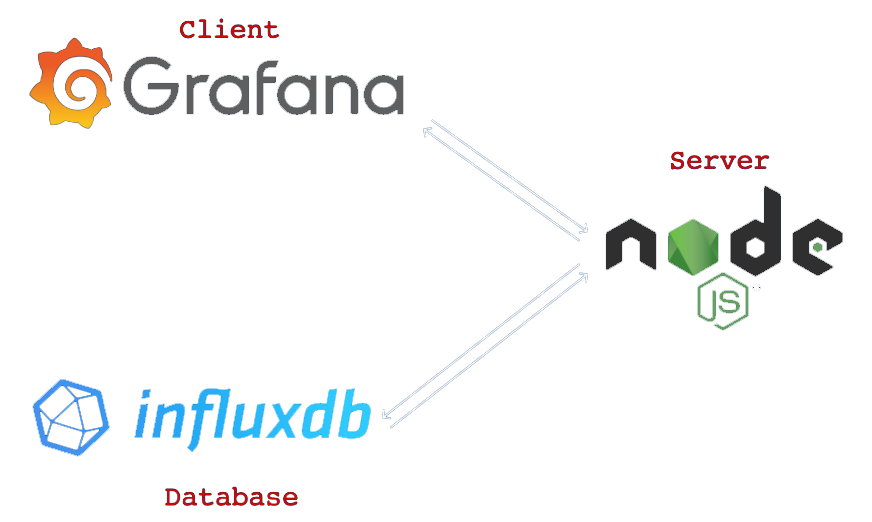
\includegraphics[scale=0.5]{./images/architettura.png} 
	\end{center}
	\caption{Architettura dell'applicativo}
\end{figure}

Il client comunica con il server attraverso il plug-in fornito dal sistema. Quest'ultimo, una volta connesso al server NodeJS il quale agirà da controller, ha a disposizione un set di funzionalità fornitoli tramite \textit{API}\glossario . Le principali mansioni del client sono le seguenti: 
\begin{itemize}
	\item Verifica dei dati: il plug-in offre all'utente la possibilità di scegliere una ristretta selezione dei dati tramite dei menù tendina, il plug-in stesso eseguirà una prima verifica dei dati inseriti;
	\item Visualizzazione dei dati: il plug-in fornisce la funzionalità incorporata di visualizzazione della rete in monitoraggio, mostrando a pannello una rappresentazione grafica della rete selezionata attualmente in monitoraggio sul server;
	\item Gestione rete bayesiana: il plug-in prende in carico la rete bayesiana, in formato \textit{.json}, caricata dall'utente, effettuando un'iniziale verifica statica dei campi. Successivamente viene incaricato dell'aggiunta di informazioni inserite e o modificate dall'utente; 
	\item Eliminazione di reti: il plug-in richiede al server l'eliminazione di una rete scelta dall'utente. 
\end{itemize}
La parte del controller e demandata al server, il quale ha il compito di filtrare le richieste ricevute dai vari plug-in connessi ad esso, salvare le reti bayesiane caricate verificandone la sintassi, calcolare le probabilità delle reti a seconda delle politiche temporali inserite e scrivere sul modello i dati calcolati. 
Fornisce delle api con le quali i vari plug-in possono interfacciarsi al server e modella la connessione al modello nel quale salvare i dati. \\ 
L'ultimo componente é il modello rappresentato dal database. Di default il prodotto arriva con la possibilità di interfacciarsi a un database
di tipo InfluxDB. L'estensibilità o l'aggiunta del modello viene rimandata al paragrafo §\ref{Estensione_Server}


\subsubsection{UML}
\begin{landscape}
\begin{figure}[H]
	\begin{center}
		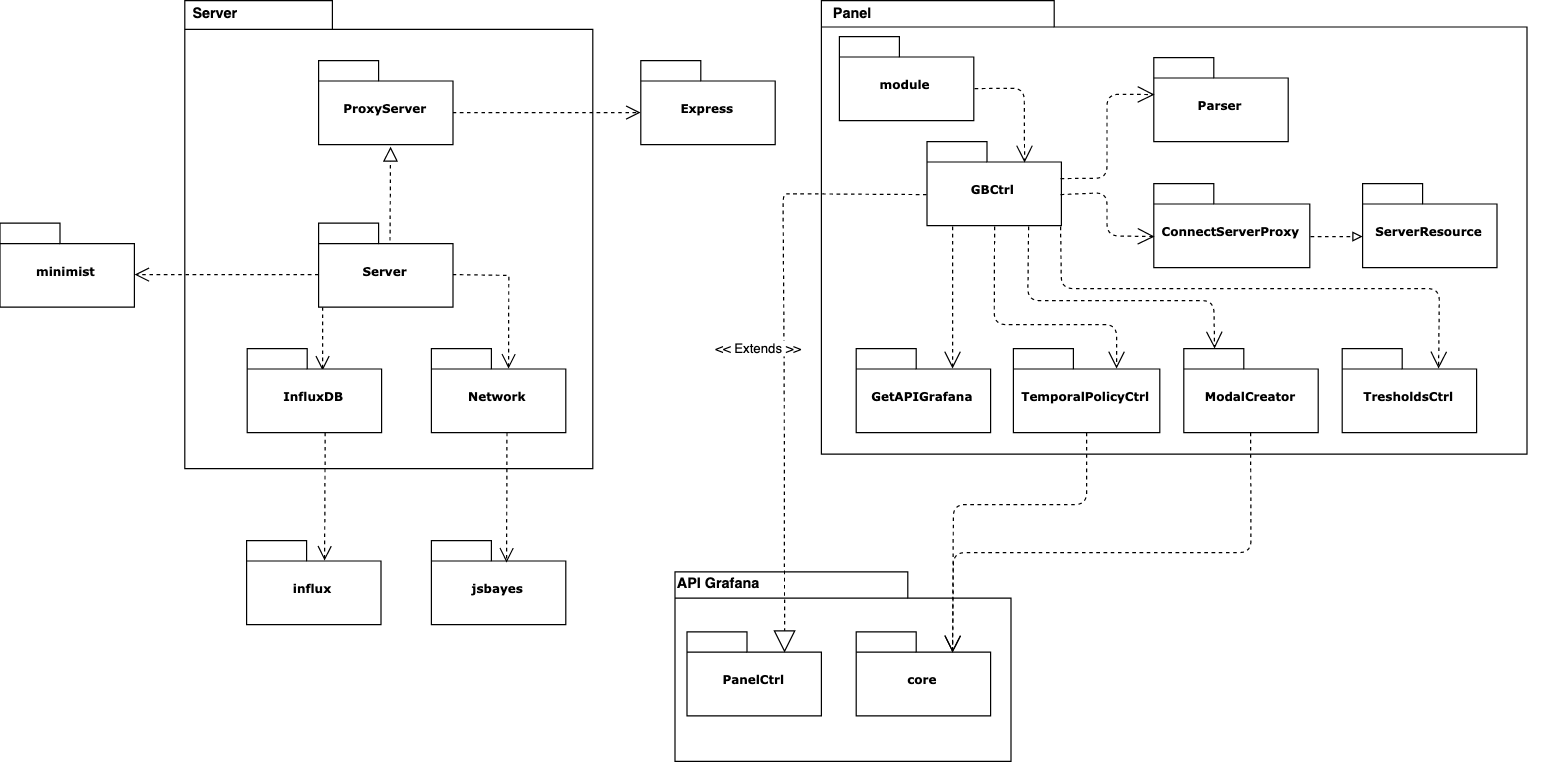
\includegraphics[scale=0.44]{./images/packageClassi.png} 
	\end{center}
	\caption{Diagramma di package dell'applicativo}
\end{figure}
\end{landscape}


 \subsection{Pannello}\label{archPannello}
Per rendere lo sviluppo più semplice, e garantire la manutenibilità del codice il team ha optato per un approccio modulare. In questo modo, avendo moduli separati con compiti distinti, sarà più semplice modificarne o estenderne il comportamento senza dover necessariamente modificare la base comune.\\
%  Il seguente diagramma delle classi mostra le relazioni tra i vari moduli. 


\subsubsection{UML}
\begin{figure}[H]
	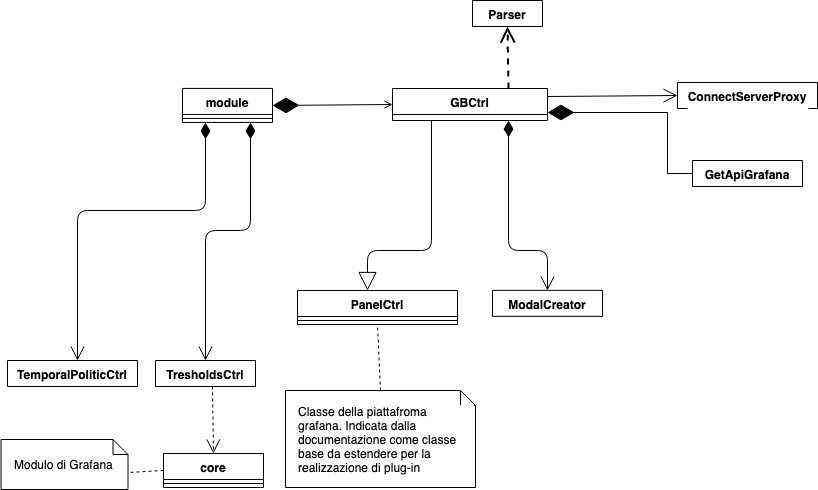
\includegraphics[width=\textwidth]{./images/plugin_non_espanso.png}
	\caption{Diagramma delle classi del Pannello}
\end{figure}

\begin{itemize}
	\item \textbf{GBCtrl}: è il modulo principale del plug-in, considerato come \textit{"main"} dall'ecosistema grafana, viene utilizzato per inizializzare l'intero panello; 
	\item \textbf{TemporalPolicyCtrl}: è il modulo che si occupa di gestire ed impostare le politiche temporali all'interno del pannello;
	\item \textbf{ThresholdsCtrl}: è il modulo che si occupa di gestire ed impostare le soglie per il monitoraggio;
	\item \textbf{Parser}: è il modulo che si occupa di controllare e interpretare la rete bayesiana in input, in formato \textit{JSON};
	\item \textbf{ConnectServer}: è il modulo che si occupa di inoltrare le richieste al Server;
	\item \textbf{ModalCreator}: è il modulo che si occupa di visualizzare le finestre che permettono l'interazione con l'utente;
	\item \textbf{ModalCreator}: è il modulo che si occupa della creazione e visualizzazione dinamica di finestre, le quali permettono l'interazione con l'utente: 
	\item \textbf{GetAPIGrafana}: è il modulo che si occupa di interagire con le API di \textit{Grafana} per ottenere i dati relativi alle sorgenti dati.
\end{itemize}

\subsubsection{Descrizione delle Classi e dei Metodi del Pannello}\label{classiPannelloDescrizione}
	
	  \paragraph{GBCtrl} 
		\begin{itemize}
			\item \textbf{resetData()} : metodo usato per riportare lo stato del pannello a prima che venga caricata una rete. Viene usato quando si deve caricare una nuova rete per eliminare le precedenti impostazioni;
			\item \textbf{resetTresholds()} : metodo usato per preparare il pannello a salvare le soglie di una nuova rete. Elimina le soglie precedenti e imposta il dizionario coi nodi della nuova rete;
			\item \textbf{checkIfAtLeastOneTresholdDefined()} : controlla se l'utente ha definito almeno una soglia, viene invocato al momento dell'inizio del monitoraggio;
			\item \textbf{deleteLinkToFlush(node)} : cancella il collegamento di un nodo ad un flusso dati e ne cancella le soglie. Viene richiamato quando l'utente clicca sul pulsante "Scollega Nodo";
			\item \textbf{freeAllFlushes()} : elimina tutti i collegamenti ai flussi e riaggiunge i flussi a quelli disponibili da scegliere. Viene invocato dal metodo \textit{resetData()};
			\item \textbf{getDatabases()} : metodo invocato al momento della creazione del pannello per ottenere da \textit{Grafana} i database disponibili;
			\item \textbf{getConnectionToDb()} : metodo che crea l'oggetto per ottenere i dati sui flussi dal database. Viene invocato al momento del collegamento al database;
			\item \textbf{checkIfConnectableToDB()} : metodo che verifica se ci si possa connettere al database selezionato, verificando: che la rete non sia sotto monitoraggio, sia stato selezionato un database e che il database selezionato sia di tipo influxdb;
			\item \textbf{getFlushes()} : metodo usato per ottenere i flussi dal database selezionato. Viene invocato quando ci si collega al database  o si carica una rete salvata nel Server;
			\item \textbf{connectToDB()} : metodo che effettua il collegamento al database. Viene invocato quando l'utente preme il pulsante "Conferma" per selezionare il database;
			\item \textbf{showTresholdModal(node)} : metodo invocato quando l'utente preme sul nome di un nodo. Fa apparire la modal per impostare le soglie;
			\item \textbf{selectTemporalPolicy()} : metodo invocato quando l'utente preme sul pulsante "Imposta" che fa apparire la modal per impostare la politica temporale;
			\item \textbf{visualizeMonitoring()} : metodo invocato quando l'utente preme il pulsante "Visualizza Monitoraggi Attivi", che fa cambiare la schermata per visualizzare i monitoraggi;
			\item \textbf{visualizeSettings()} : metodo invocato quando l'utente preme il pulsante "Visualizza Impostazioni", per tornare alla schermata delle impostazioni della rete;
			\item \textbf{splitMonitoringNetworks()} : metodo invocato quando vengono richieste le reti al Server. Si preoccupa di capire quali sono sotto monitoraggio e di suddividerle correttamente;
			\item \textbf{requestNetworks()} : metodo invocato ogni volta che viene salvata una rete sul Server e quando ci si collega ad esso. Richiede la lista delle reti al Server;
			\item \textbf{tryConnectServer()} : metodo per provare a vedere se il Server è online su porta e ip specificati. Viene invocato quando l'utente preme sul tasto "Connetti" da Server Settings;
			\item \textbf{checkIfNetworkIsDeletable(net)} : metodo che viene invocato quando l'utente preme sul tasto "Elimina" per eliminare una rete. Richiede al Server che venga eliminata la rete selezionata;
			\item \textbf{calculateSeconds(temp)} : metodo per calcolare i secondi totali della politica temporale. Viene usato dal metodo changeNetworkToVisualizeMonitoring() per impostare la politica di refresh delle probabilità;
			\item \textbf{deleteProbRefresh()} : metodo usato per eliminare l'intervallo di refresh delle probabilità. Viene invocato quando l'utente ritorna alla schermata delle impostazioni delle reti;
			\item \textbf{updateProbs()} : metodo invocato per aggiornare il disegno delle probabilità della rete. Viene invocato ad intervalli regolari stabiliti dalla politica temporale della rete;
			\item \textbf{changeNetworkToVisualizeMonitoring()} : metodo invocato quando l'utente seleziona una nuova rete di cui visualizzare le probabilità. Imposta il timer di refresh delle probabilità e aggiorna il disegno della rete;
			\item \textbf{buildDataToSend()} : metodo invocato quando bisogna salvare una rete sul Server. Costruisce il pacchetto contenente tutti i dati necessari da salvare;
			\item \textbf{loadNetworkToServer(net)} : metodo usato per salvare una rete sul Server;
			\item \textbf{saveActualChanges()} : metodo invocato quando viene caricata una rete. Verifica se era già presente una rete e se essa abbia bisogno di essere salvata sul Server. In caso positivo la salva prima di caricare quella nuova;
			\item \textbf{requestNetworkToServer(net)} : metodo invocato quando l'utente preme il pulsante "Apri" per caricare una rete salvata nel Server. Si occupa di caricare nel pannello le informazioni della rete e di collegarsi al database corretto;
			\item \textbf{loadNetworkFromSaved(net)} : metodo usato quando l'utente carica una rete da quelle salvate. Si occupa di assegnare le variabili;
			\item \textbf{loadNetwork(data)} : metodo invocato quando l'utente clicca sul pulsante per confermare la rete da caricare dalla memoria locale. Si preoccupa verificare che la rete sia corretta e di inizializzarla;
			\item \textbf{panelPath()} : metodo per ottenere il percorso del pannello;
			\item \textbf{checkIfCanStartComputation()} : metodo che verifica se l'utente ha correttamente impostato i parametri per far partire la computazione;
			\item \textbf{startComputation()} : metodo invocato quando l'utente preme sul pulsante "Avvia Monitoraggio". Esso fa partire la computazione e salva la rete nel Server;
			\item \textbf{closeComputation()} : metodo invocato quando l'utente preme sul pulsante "Interrompi Monitoraggio" per interrompere il monitoraggio.
	\end{itemize}
	  \paragraph{TemporalPolicyCtrl} 
			\begin{itemize}
				\item	\textbf{checkCorrectData()} : metodo che verifica la correttezza dei dati inseriti per la politica temporale;
				\item \textbf{setConfirmationToTrue()} : metodo invocato quando l'utente preme sul tasto "Conferma" dalla modal della politica temporale. Verifica che sia stata impostata correttamente e lo notifica al pannello, facendo anche sparire la modal;
				\item \textbf{setConfirmationToFalse()} : metodo invocato quando l'utente modifica la politica temporale  per notificare al pannello che al momento non è valida.
	\end{itemize}
				  \paragraph{TresholdsCtrl}
			\begin{itemize}
				\item \textbf{checkIfTherIsAtLeastOneTreshold(node)} : verifica che l'utente abbia impostato almeno una soglia. Viene invocato dal metodo \textit{confirmTresholdsChanges(node)} per verificare che l'utente abbia definito almeno una soglia;
				\item \textbf{checkNotRepeatedTresholds(node)} : verifica che l'utente non abbia definito soglie ripetute. Viene invocato dal metodo \textit{confirmTresholdsChanges(node)};
				\item \textbf{splitForSign(node)} : divide le soglie per segno. Viene invocato per verificare che non ci siano conflitti tra le soglie;
				\item \textbf{setError(value1, value2, sign1, sign2)} : metodo invocato da tutti gli altri metodo qual ora vi sia un errore. fa apparire una modal con l'errore;
				\item \textbf{checkConflictMin(min, maj, maje)} : verifica che non ci siano conflitti tra le soglie "<" con le soglie ">" e ">=". Viene in vocato dal metodo\textit{checkConflicts(data)};
				\item \textbf{checkConflictMine(mine, maj, maje)} : verifica che non ci siano conflitti tra le soglie "<=" con le soglie ">" e ">=". Viene in vocato dal metodo\textit{checkConflicts(data)};
				\item \textbf{checkConflictSameSign(arr1, arr2, sign1, sign2)} : verifica che non ci siano conflitti tra le soglie con lo stesso segno. Viene in vocato dal metodo\textit{checkConflicts(data)};
				\item \textbf{checkConflicts(data)} : si occupa di invocare tutti i metodi per verificare la presenza di conflitti tra le soglie. Viene invocato dal metodo \textit{confirmTresholdsChanges(node)};
				\item \textbf{associate(node)} : crea l'associazione tra il nodo e il flusso attualmente selezionato. Viene invocato dal metodo \textit{confirmTresholdsChanges(node)}.
				\item \textbf{confirmTresholdsChanges(node)} : metodo invocato quando l'utente preme sul tasto "Conferma" dalla modal della politica temporale. Invoca tutti i metodi per verificare la correttezza delle soglie e crea le associazioni qual ora necessario;
				\item \textbf{addTreshold(node, state)} : metodo invocato quando l'utente preme un tasto per aggiungere una soglia al nodo. Aggiunge la soglia relativa allo stato a cui si riferisce;
				\item \textbf{deleteTreshold(node, name)} : metodo invocato quando l'utente preme su un tasto "Remove" dalla modal delle soglie. Rimuove la soglia corrispondente;
				\item \textbf{setNotLinked(node)} : rimuove il collegamento tra il nodo e il flusso. Viene invocato quando l'utente esegue una qualsiasi azione diversa dal confermare le soglie dalla modal delle soglie;
				\item \textbf{setLinked(node)} : imposta il nodo come collegato. Viene invocato dal metodo \textit{confirmTresholdsChanges(node)};
			\end{itemize}
		
		 \paragraph{Parser} 
			\begin{itemize}
				\item \textbf{validateNet()} : invoca tutti i metodi per verificare la correttezza della rete;
				\item \textbf{checkMinimumFields()} : verifica che il file \textit{.JSON} abbia il numero corretto di campi, i quali devono avere anche il nome corretto;
				\item \textbf{checkNamedNodes(data, field)} : verifica che il campo data abbia il corretto numero di linee e che esse abbiano il nome giusto;
				\item \textbf{checkDuplicates(values)} : verifica che nell'array values non ci siano valori duplicati. Viene invocato dal metodo \textit{checkParents()} per verificare che non ci siano padri ripetuti;
				\item \textbf{checkStates()} : verifica che gli stati dei nodi siano correttamente definiti;
				\item \textbf{checkParents()} : verifica che i padri dei nodi siano correttamente definiti;
				\item \textbf{checkProbabilities()} : verifica che le probabilità dei nodi siano correttamente definiti;
				\item \textbf{countNumberOfValue(node)} : metodo usato da \textit{checkProbabilities()} per verificare che ogni nodo abbia il numero corretto di probabilità. Calcola quante probabilità il nodo deve avere sulla base degli stati e dei padri.
			\end{itemize}
				  \paragraph{ConnectServer}
			\begin{itemize}
				\item \textbf{alive()} : verifica che il Server sia online su porta e ip specificati. Viene invocato quando dal metodo \textit{tryConnectServer()} di \textit{GBCtrl};
				\item \textbf{networks()} : richiede al Server le reti salvate. Viene invocato da \textit{GBCtrl} in molteplici punti;
				\item \textbf{uploadnetwork(net)} : effettua la richiesta al Server per salvare la rete net passata come parametro. Viene invocato da \textit{GBCtrl};
				\item \textbf{deletenetwork(net)} : effettua la richiesta al Server per eliminare la rete net passata come parametro. Viene invocato da \textit{GBCtrl} nel metodo \textit{requestNetworkDelete(net)};
				\textit{getnetworkprob(net)} : effettua la richiesta al Server per ottenere il graph della libreria \textit{JSBayes} relativo alla rete net. Viene invocato dal metodo \textit{updateProbs()} di \textit{GBCtrl} per rinnovare le probabilità della rete sotto monitoraggio;
				\item \textbf{getnetwork(net)} : effettua la richiesta al Server per ottenere i dati della rete di nome specificato nel parametro net. Viene invocato in vari punti da \textit{GBCtrl}.
			\end{itemize}
				  \paragraph{ModalCreator}
			\begin{itemize}
				\item \textbf{checkMonitoring(message)} : verifica se la rete attuale è sotto monitoraggio e in caso positivo fa apparire il messaggio di errore. Viene invocato da \textit{showTresholdModal(node) e selectTemporalPolicy()};
				\item \textbf{checkDB(message)} : verifica che il pannello sia collegato ad un database e in caso negativo fa apparire un messaggio di errore. Viene invocato da \textit{showTresholdModal(node) e selectTemporalPolicy()};
				\item \textbf{showMessageModal(message, title)} : fa apparire una modal con il messaggio di errore message e titolo title. Viene invocato dagli altri metodi;
				\item \textbf{showTresholdModal(node)} : metodo invocato da \textit{GBCtrl} per far apparire la modal per definire le soglie del nodo node;
				\item \textbf{selectTemporalPolicy()} : metodo invocato dal metodo \textit{selectTemporalPolicy()} di \textit{GBCtrl} per far apparire la modal per la definizione della politica temporale.
			\end{itemize}
				  \paragraph{GetApiGrafana}
			\begin{itemize}
				\item \textbf{queryAPI()} : metodo invocato dal metodo \textit{getData()} per ottenere i database disponibili da \textit{Grafana};
				\item \textbf{getData()} : metodo invocato dal metodo \textit{getDatabases()} di \textit{GBCtrl} per ottenere la lista dei databse ben strutturata;
				\item \textbf{getDatasources()} : ritorna i flussi disponibili dal database selezionato ben strutturati. Viene invocato dal metodo \textit{getFlushes()} di \textit{GBCtrl};
				\item \textbf{getTables()} : richiede a \textit{Grafana} le tabelle del database selezionato. Viene invocato dal metodo \textit{getDatasources()};
				\item \textbf{getFields(tables)} : richiede a \textit{Grafana} i campi delle tabelle specificate nel parametro tables. Viene invocato dal metodo \textit{getDatasources()};
				\item \textbf{divideFields(elements)} : metodo invocato da \textit{getDatasources()} per formattare correttamente i dati sui campi delle tabelle ottenuti da \textit{Grafana};
				\item \textbf{initialize()} : metodo invocato da \textit{getDatasources()} per interpretare correttamente il link del database.
			\end{itemize}

\newpage

\subsection{Server}\label{archServer}
Per rendere lo sviluppo più semplice, e garantire la manutenibilità del codice il team ha optato per un approccio modulare. In questo modo, avendo moduli separati con compiti distinti, sarà più semplice modificarne o estenderne il comportamento senza dover necessariamente modificare la base comune.\\

\subsubsection{UML}
\begin{figure}[H]
	\begin{center}
		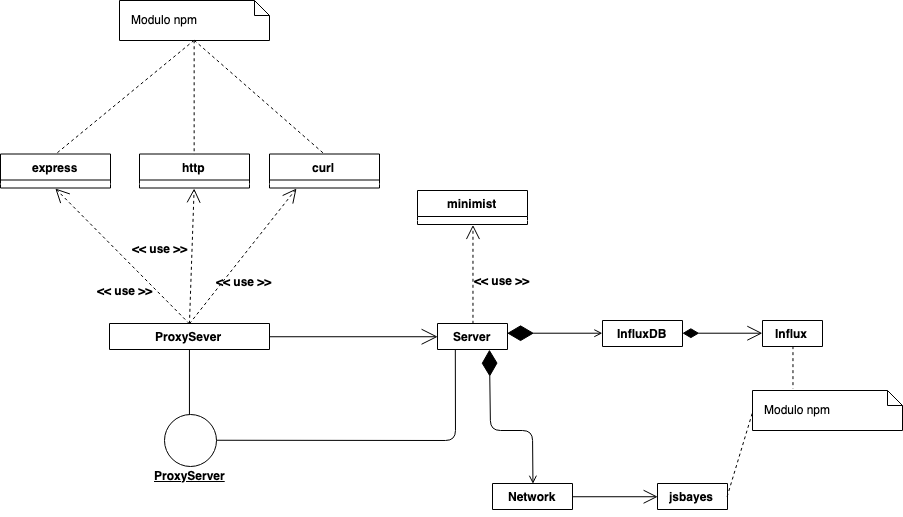
\includegraphics[scale=0.5]{./images/server_class_non_espanso.png} 
	\end{center}
	\caption{Architettura dell'applicativo}
\end{figure}

\begin{itemize}
 \item \textbf{Server}: è il modulo principale che si occupa di comunicare con gli altri, ed esegue le operazioni fondamentali;
 \item \textbf{InfluxDB}: è il modulo che si occupa di adattare la libreria \textit{Influx} e ci fornisce un set di metodi specializzati;
 \item \textbf{Network}: è il modulo che si occupa di adattare la libreria \textit{jsbayes} e costruisce la rete bayesiana da utlizzare;
 \item \textbf{ProxyServer}: è il modulo che si occupa di filtrare, autenticare le richieste verso il server e  protegge lo stesso.
\end{itemize}

\subsubsection{Descrizione delle Classi e dei Metodi del Pannello}\label{descrizionearchServer}

\paragraph{Server}

\begin{itemize}

	\item \textbf{constructor()}: costruttore di classe. Inizializza l'istanza di express\glossario , l'array di
	 connessioni, reti e di pool, inoltre esegue una verifica sintattica sui parametri di configurazioni passati 
	 tramite \textit{conf.json};

	 \item \textbf{configExpressApp()}: metodo utilizzato per l'inizializzazione delle varie route\glossario messe 
	 a disposizione dal server;

	 \item \textbf{parserNetworkNameURL(name)}: metodo utilizzato per parsare il nome di una rete 	
	 proveniente da indirizzo URL. 
	 Ritorna false in caso di errore o stringe non valide, altrimenti ritorna il nome parsato;

	 \item \textbf{saveNetworkToFile(data)}: metodo utilizzato per il salvataggio su filesystem delle reti 
	 bayesiane caricate dall'utente. Riceve come input un json rappresentate la rete bayesiana. Ritorna un 	
	 booleano a true se il salvataggio è stato eseguito o false altrimenti. Lancia eccezioni in caso di errori di 
	 scrittura su filesystem;

	 \item \textbf{startServer()}: metodo utilizzato per l'effettivo avvio del server. Mette in ascolto il server 
	 sulla porta configurata a costruttore ed inizializza le reti salvate su filesystem; 

	 \item \textbf{shutDown()}: metodo utilizzato per la chiusura del server; 

	 \item \textbf{initSavedNetworks()}: metodo utilizzato per  la lettura da file system e il successivo
	 caricamento in memoria  delle reti bayesiane salvate in filesystem. Per ogni rete letta, viene chiamato
	 il metodo \textit{initBayesianNetwork(net)};

	 \item \textbf{initDatabaseConnection(connection)}: metodo utilizzato per l'inizializzazione di una 
	 connessione al database. Riceve come parametro un json di definizione della connessione da creare. 
	 Può lanciare un'eccezione in caso di fallimento;

	 \item \textbf{initBayesianNetwork(net)}: metodo utilizzato per aggiungere un'istanza di \textbf{Network}
	 all'array di reti monitorate. Riceve in input la definizione della rete in json, e ne crea l'oggetto che la rappresenta; Può lanciare eccezioni. Ritorna true se la creazione è andata a buon fine; 

	\item \textbf{countNetworks()}: ritorna in numero di reti nell'array di reti monitorate; 

	\item \textbf{observeNetworks(net, data)}: metodo utilizzato per risolvere le dependency richiesta
	dall'oggetto \textit{Network} per eseguire il calcolo delle probabilità. Riceve in input la rete da osservare
	e i dati richiesti da quest'ultima. Successivamente esegue una chiamata al database chiedendo i dati 
	necessari al calcolo per poi eseguire i calcoli con quest'ultimi chiamando il metodo apposito. Inoltre 
	il metodo è incaricato della gestione delle soglie critiche modificando qualora fosse necessario 
	la politica temporale di ricalcolo. Fine richiama il metodo \textit{writeMesure(net)}; 

	\item \textbf{configParser()}: metodo utilizzato per il controllo  della sintassi nel file di configurazione; 
	Ritorna true se la sintassi è corretta, false altrimenti; 

	\item \textbf{checkParam(argv)}: metodo utilizzato per il controllo dei parametri passati da terminale
	all'avvio del server. Ritorna true se i parametri sono validi, false altrimenti; 

	\item \textbf{getNetworks()}: metodo utilizzato per la creazione di un'array contenente il nome e 
	il campo \textit{monitoring} di tutte le reti salvate in filesystem; Ritorna un'array di tuple stringa, boolean; 

	\item \textbf{getMilliseconds(temporal)}: metodo utilizzato per la conversione della politica temporale in 
	ore, minuti, secondi in millisecondi. Riceve in input un json con ore, minuti e secondi definiti come interi, 
	e ritorna un intero, il quale rappresenta la conversione in millisecondi; 

	\item \textbf{addToPool(net)}: metodo utilizzato per aggiungere al monitoraggio una rete bayesiana già 
	caricata in memoria. Riceve come parametro il nome della rete, con quest'ultimo viene verificato 
	se è gia presente nel all'array di pool. Se non è presente viene aggiunto al pool seguendo le politiche 
	temporali riportate dall'utente. Ritorna true nel caso in cui la rete sia stata aggiunta con successo, false 
	altrimenti; 

	\item \textbf{deleteFromPool(net)}: metodo utilizzato per l'eliminazione di una rete in monitoraggio. Riceve
	come parametro il nome della rete. Se la rete è in monitoraggio viene fermata ed eliminata dal pool; 
	Ritorna true se la rete è stata eliminata dal pool di monitoraggio, false altrimenti; 
	
	\item \textbf{writeMesure(net)}: metodo utilizzato per la scrittura delle probabilità calcolate dalla
	varie reti in monitoraggio sui rispetti database di salvataggio. Riceve in input il nome di una rete, 
	dopodiché preleva le probabilità calcolate dall'oggetto rappresentate la rete e le scrive sul database. 
	Ritorna true se i dati sono stati scritti con successo, false altrimenti; 
	
\end{itemize}

\paragraph{Network}
\begin{itemize}

	\item \textbf{constructor(net)}: costruttore di classe a un parametro. Riceve la definizione di una rete 
	bayesiana in formato JSON e ne costruisce l'oggetto rappresentate; 

	\item \textbf{observe(node, state)}: metodo utilizzato da wrap\glossario per l'utilizzo del metodo 
	\textit{observe} della classe \textit{jsbayes}. Riceve in input due parametri: net	di tipo stringa e state di 
	tipo stringa; 

	\item \textbf{sample(n)}: wapper\glossario del metodo \textit{sample(n)}, della classe \textbf{jsbayes}. 
	Esegue il calcolo delle probabilità dei vari nodi con il metodo \textit{Monte Carlo}. Riceve in input un 
	numero intero il quale indica il numero di iterazioni da eseguire; 
	
	\item \textbf{unobserveAll()}: metodo utilizzato per togliere dall'osservazione i vari nodi precedentemente 
	collegati. Per ogni nodo viene richiamato il metodo \textit{unobserve(node)} della classe jsbayes; 
	
	\item \textbf{orderTresholds()}: metodo utilizzato per il riordinamento delle soglie, in ordine crescente e 
	decrescente, definite nella rete; 
	
	\item \textbf{observeData(dati)}: metodo utilizzato per l'osservazione dei dati. Riceve in input un'array 
	associativo dei dati necessari da monitorare, tramite i quali verranno effettuate a seconda delle 
	soglie, i confronti tra dati - soglie, per poi successivamente fare scattare la probabilità con li metodo 
	\textit{observe}. In finte una volta eseguiti tutti i confronti verrà richiamato il metodo \textit{sample} per 
	calcolare le probabilità. Ritorna true se una soglia critica è stata superata, false altrimenti; 
	
	\item \textbf{getProbabilities()}: metodo utilizzato per estrarre le probabilità di ogni stato, per ogni 
	singolo nodo. Ritorna un'array associativo con il nome del nodo e un array contenete le probabilità. 
	Quest'ultimo a sua volta è un'array associativo formato da tuple: nome stato e probabilità calcolata; 
			
\end{itemize}

\paragraph{InfluxDB}

\begin{itemize}

	\item \textbf{constructor(host, port, database, dbwrite, user, pwd)}: costruttore di classe. Riceve in 
	input host e porta sulla quale il database è in ascolto, il nome del database, il database sul quale salvare i 
	dati, username e password. Il metodo costruisce un oggetto \textit{Influx} il quale rappresenta la 
	connessione al database. Avviene un controllo dei dati passati input con opportuno lancio di eccezioni 
	nel caso in cui alcuni dei dati non fossero conformi alla sintassi o errati; 
	
	\item \textbf{getDatasources()}: metodo utilizzato per estrapolare le tabelle disponibili per la lettura.
	Ritorna una \textit{Promise} da risolvere successivamente. Può lanciare un'eccezione nel caso in cui 
	la query\glossario al database fallisca o sia interrotta; 
	
	\item \textbf{queryDB(query)}: wrapper del metodo \textit{query} della classe \textit{InfluxDB}, il quale
	viene utilizzato per l'interrogazione del database tramite query; 
	
	\item \textbf{getDatasourcesFields(source)}: metodo utilizzato per estrarre le colonne di una determinata 
	tabella. Riceve in input una source da ispezionare. Ritorna una \textit{Promise} da risolvere
	successivamente; 
	
	\item \textbf{getLastValue(source, field)}: metodo utilizzato per leggere l'ultimo dato in serie temporale 
	dal database. Riceve in input la source dalla quale estrarre il field interessato. Ritorna una \textbf{Promise}
	da risolvere successivamente. Può lanciare un'eccezione nel caso in cui l'interrogazione del database 
	fallisca; 
	
	\item \textbf{getListData(fields)}: metodo utilizzato per generare un'array di ultimi dati, prelevati 
	in serie temporali dal database. Riceve in input un'array di json, nel quale per ognuno di essi viene 
	definito un campo table ed un campo flush. Per ogni valore da prelevare viene richiamato il metodo 
	\textit{getLastValue} per ricevere l'ultimo dato in ordine temporale. 
	Ritorna un'array di tuple: nome campo  e valore campo; 
	
	\item \textbf{writeOnDB(net, probs)}: metodo utilizzato per la scrittura delle probabilità di una rete sul
	database di scrittura definito in fase di costruzione. Riceve in input il nome della rete e le sue probabilità. 
	Per ogni nodo della rete viene inserito un campo contenente il nome del nodo e le varie probabilità
	calcolate; 
	
	\item \textbf{checkStatus(timeout)}: metodo utilizzato per verificare la connessione al database. 
	Riceve in input un timeout utilizzato per effettuare un ping\glossario al database ogni 
	\textit{timeout} secondi. Ritorna un \textit{Promise} da risolvere successivamente la quale 
	contiene i dati di risposta dal database; 

\end{itemize}










